\chapter{Risultati e loro discussione} 
\label{ch:risultatiediscussione} 

Nella sezione n° \ref{ch:risultatiediscussione} verranno illustrati e discussi alcuni dei risultati più significativi ottenuti dall'applicazione dei metodi esposti (vedi Sez.\ref{ch:materialandmethods}) per il calcolo del ranking, rispettivamente delle stazioni e delle tratte ferroviarie.
Per i risultati completi si rimanda alla lettura dell'appendice \ref{risultati}.
\section{Ranking e  Valutazione delle stazioni ferroviarie}

Applicando il metodo discusso nella Sez. \ref{metodoNuovo} abbiamo ottenuto i risultati che andremo qui di seguito ad illustrare.
Tali risultati sono stati utilizzati per realizzare una classifica delle stazioni in base al loro grado di esposizione al pericolo idrogeologico.

%inserire parte introduttiva che richiama i dati in analisi a quale tabella/colonna appartengono della bd..

Il valore di \textit{exposure} ottenuto per le stazioni in analisi  varia da un valore minimo di $0$ ad un massimo di $50$. A fronte di tali risultati si è deciso di definire tre diverse fasce di esposizione al pericolo in base alle quali aggregare le stazioni all'interno della classifica:
\begin{itemize}
\item \textit{High}
\item \textit{Moderate}
\item \textit{Low}
\end{itemize}
La Tabella n°\ref{range} mostra la suddetta suddivisione in fasce di rischio, gli intervalli in cui le stazioni sono state divise secondo il valore di \textit{exposure}, il numero e la percentuale sul totale delle stazioni appartenenti ad una determinata fascia. Inoltre ad ogni fascia è stato associato un colore identificativo.
\begin{table}[h]
\centering
\begin{tabular}{|c|c|c|c|}
\hline
\rowcolor{lightgray}
\textbf{Fascia} & \textbf{Intervallo valori Exp$\mathbf{\_}$$\mathbf{b_i}$} & $\mathbf{\#b_i}$ & \textbf{\%} \\
\hline
\rowcolor{flamingopink}
High & 20 < Exp$\_$$b_i$ < 50 & 6 & 5,26\%\\
\hline
\rowcolor{icterine}
Moderate & 1 < Exp$\_$$b_i$ < 20 & 62 & 54,39\%\\
\hline
\rowcolor{inchworm}
Low & $0$ < Exp$\_$$b_i$ < 1 & 46 & 40,35\%\\
\hline
\end{tabular}
\caption{Aggregazione delle stazioni $b_i$ in base al valore di \textit{exposure} }
\label{range}
\end{table}

Come si evince dalla tabella \ref{range} tale suddivisione in fasce non è lineare ma bensì frutto di un'analisi critica (vedi Sez.  \ref{analisicritica}) del metodo discusso (vedi Sez. \ref{metodoNuovo}) e dei risultati ottenuti. Inoltre è possibile notare come la maggioranza delle stazioni presenta un livello di esposizione al rischio \textit{Moderate} mentre solo il 5,26\% presenta valori di \textit{exposure} tali da far emergere il bisogno di controlli più frequenti (fascia \textit{High}).

Nella tabella \ref{classifica} si riportano i primi dieci record, appartenenti alla classifica delle stazioni ordinati in modo decrescente rispetto il valore di \textit{exposure}. In riferimento alla singola stazione, per ogni record vengono quindi mostrati la posizione all'interno della classifica, l'identificativo, il nome e il suo valore di \textit{exposure}.

\begin{table}[h]
\centering
\begin{tabular}{|c|c|c|c|}
\hline
\rowcolor{lightgray}
\textbf{n.} & \textbf{id Stazione} & \textbf{Nome Stazione Ferroviaria} & \textbf{Valore di \textit{exposure}} \\
\hline
\rowcolor{flamingopink}
1 & 114 & Acciano & 49,85 \\
\hline
\rowcolor{flamingopink}
2 & 54 & Fontecchio & 42,68 \\
\hline
\rowcolor{flamingopink}
3 & 44 & Sant'Ilario & 31,73 \\
\hline
\rowcolor{flamingopink}
4 & 38 & Pettorano Sul Gizio & 31,14 \\
\hline
\rowcolor{flamingopink}
5 & 94 & Isca d'Archi & 22,71 \\
\hline
\rowcolor{flamingopink}
6 & 66 & Prezza & 20,54 \\
\hline
\rowcolor{icterine}
7 & 33 & Bussi & 19,98 \\
\hline
\rowcolor{icterine}
8 & 81 & Capistrello & 18,57 \\
\hline
\rowcolor{icterine}
9 & 91 & Civitaluparella & 16,32 \\
\hline
\rowcolor{icterine}
10 & 63 & Sella di Corno & 14,24 \\
\hline
\end{tabular}
\caption{Classifica delle prime dieci stazioni ordinata in base al valore di \textit{exposure}}
\label{classifica}
\end{table}
%inserire appendice dove sta la classificazione ufficiale
%discutere se inserire l'ordinamento della classifica ufficiale
\subsection{Analisi critica del Nuovo Metodo Proposto}
\label{analisicritica}
Osservando i risultati ottenuti dall'applicazione del metodo di cui abbiamo discusso nella Sez. \ref{metodoNuovo} abbiamo potuto osservare come i valori di \textit{exposure} delle stazioni ferroviarie non presentano una distribuzione\newline "\textit{omogenea/lineare}" lungo l'asse dei numeri reali bensì risultano "aggregati" in gruppi di valori i quali ci hanno guidato nella definizione dei range di valori per ogni fascia che abbiamo presentato nella Tab. \ref{range}.
Il NMC restituisce valori in , quindi utilizzare un'equazione lineare per aggregare le stazioni in 3 fasce in base al loro valore di \textit{exposure} risulterebbe errato.
Al fine di poter valutare le performance del metodo proposto nella Sez. \ref{metodoNuovo} abbiamo confrontato la classificazione in fasce delle stazioni ottenuta in base ai valori di \textit{exposure} con la classificazione in fasce delle stazioni ferroviarie presenti sul territorio realizzata dai membri dei gruppi partecipanti al Laboratorio di Basi di Dati II nell'A.A. 2016/2017 tramite un'indagine visiva del territorio ove tali edifici sono situati. L'ipotesi di lavoro implicita è che tale classificazione "umana", indicata d'ora in avanti come classificazione ufficiale, sia corretta per definizione. Pertanto i risultati ottenuti dal metodo discusso nella Sez. \ref{metodoNuovo} saranno tanto più soddisfacenti quanto più questi si avvicineranno ai dati ufficiali.

La tabella che riporta la classificazione in fasce ufficiale delle stazioni ferroviarie nella sua completezza è presente in appendice \ref{risultatiUfficiali}, mentre qui di seguito, in tabella \ref{fasciaHighUfficiale}, sono stati riportati i record delle stazioni che sono stati classificati ufficialmente in fascia \textit{High}.
\newpage
\begin{table}[h]
\centering
\begin{tabular}{|c|c|}
\hline
\rowcolor{lightgray}
\textbf{id Stazione} & \textbf{Nome Stazione Ferroviaria} \\
\hline
\rowcolor{flamingopink}
44 & Sant'Ilario \\
\hline
\rowcolor{flamingopink}
65 & Aversa \\\hline
\rowcolor{flamingopink}
54 & Fontecchio \\\hline
\rowcolor{flamingopink}
38 & Pettorano sul Gizio \\\hline
\rowcolor{flamingopink}
114 & Acciano \\\hline
\rowcolor{flamingopink}
62 & Vigliano d'Abruzzo \\
\hline
\end{tabular}
\caption{Elenco delle stazioni ferroviarie ufficialmente in fascia \textit{High}}
\label{fasciaHighUfficiale}
\end{table}

Lo studio delle performance del metodo è stato realizzato mediante la \textit{tabella di contingenza} (detta anche \textit{matrice di errore} o \textit{di confusione}). Ogni colonna di tale tabella rappresenta le istanze in una fascia "prevista" (\textit{Predicted Classes}) mentre le righe rappresentano le istanze in una fascia reale (\textit{Actual Classes}). La corrispondente \textit{tabella di contingenza} (tabella \ref{tabellaContingenza}) riassume i risultati ottenuti con il metodo. 

\begin{table}[h]
\centering
\begin{tabular}{|cc|c|c|c|c|}
\hline
\multicolumn{2}{|c|}{\multirow{2}*{}} & \multicolumn{3}{c|}{Predicted Classes} & \multirow{2}*{Totale} \\
\cline{3-5}
 & & High & Moderate & Low &  \\
\hline
\multicolumn{1}{|c|}{\multirow{3}*{Actual Classes}} & High & $4$ & $2$ & $0$ & 6 \\
\cline{2-6}
\multicolumn{1}{|c|}{}& Moderate & $2$ & $53$ & $6$ & $61$ \\
\cline{2-6}
\multicolumn{1}{|c|}{}& Low & $0$ & $7$ & $40$ & $47$ \\
\hline
\multicolumn{2}{|c|}{Totale}& $6$ & $62$ & $46$ & $114$ \\
\hline
\end{tabular}
\caption{\textit{Tabella di Contingenza} del metodo NMC discusso nella Sez. \ref{metodoNuovo}}
\label{tabellaContingenza}
\end{table}

Osservando i dati contenuti nella tabella \ref{tabellaContingenza} è possibile ricavare le seguenti deduzioni:
\begin{itemize}
\item Delle 6 stazioni classificate ufficialmente in fascia \textit{High} il metodo ha previsto che 2 di queste sono in fascia \textit{Moderate};
\item Delle 61 stazioni classificate ufficialmente in fascia \textit{Moderate} il metodo ha previsto che 2 di queste sono in fascia \textit{High} mentre 6 sono in fascia \textit{Low};
\item Delle 47 stazioni classificate ufficialmente in fascia \textit{Low} il metodo ha previsto che 7 sono in fascia \textit{Moderate};
\item Le stazioni correttamente classificate dal nostro metodo sono localizzate lungo la diagonale della tabella.
\end{itemize}

Dall'esame della \textit{letteratura} del settore del \textit{Machine Learning} emerge che la maniera più semplice di effettuare misurazioni circa le performance della predizione restituita dal metodo adottato consiste nel ricondurre il problema della classificazione dei risultati ottenuti al caso di \textit{tabella di contingenza binaria}, ossia al caso nel quale sia coinvolta una sola classe alla volta. Il problema può essere quindi formulato come segue:
\newline
\newline
\textit{Dati n valori (v1, v2, …, vn) e una classe (C), costruire la tabella di contingenza binaria che riassume
come detti valori sono classificati sia nel mondo reale che secondo quanto stimato dall’algoritmo del
quale si vuole misurare la efficacia. Evidentemente il valore v1 potrà cadere in C oppure no, idem per
v2, …., vn.}
\newline
\newline
Dalla tabella \ref{tabellaContingenza} è possibile ricavare le seguenti \textit{tabelle di contingenza} riferite relativamente alla fascia \textit{High} (Tabella \ref{tabellaHigh}), alla fascia \textit{Moderate} (Tabella \ref{tabellaModerate}) e alla fascia \textit{Low} (Tabella \ref{tabellaLow}).

\begin{table}[h]
\centering
\begin{tabular}{|cc|c|c|c|}
\hline
\multicolumn{2}{|c|}{\multirow{2}*{}} & \multicolumn{2}{c|}{Predicted Classes} & \multirow{2}*{Totale} \\
\cline{3-4}
 & & High & Not High &  \\
\hline
\multicolumn{1}{|c|}{\multirow{2}*{Actual Classes}} & High & $4$  & $2$ & 6 \\
\cline{2-5}

\multicolumn{1}{|c|}{}& Not High  & $2$ & $106$ & $108$ \\
\hline
\multicolumn{2}{|c|}{Totale}& $6$ & $108$ & $114$ \\
\hline
\end{tabular}
\caption{\textit{Tabella di contingenza binaria} riferita alla fascia \textit{High} }
\label{tabellaHigh}
\end{table}

\textbf{Segue un commento alla tabella \ref{tabellaHigh}}

Prima Riga:
\begin{itemize}
\item Il numero 4 denota le stazioni che il metodo ha classificato correttamente in fascia \textit{High} (da questo
momento chiameremo questi casi \textit{Veri Positivi});
\item Il numero 2 denota le stazioni che il metodo \textbf{non} ha classificato \textbf{correttamente} in fascia \textit{High} ma in un'altra fascia  (da questo momento chiameremo questi casi \textit{Falsi
Negativi}).
\end{itemize}

Seconda Riga:
\begin{itemize}
\item Il numero 2 denota i casi nei quali l’algoritmo ha classificato \textbf{erroneamente} delle stazioni in classe \textit{High} (da
questo momento chiameremo questi casi \textit{Falsi Positivi});
\item Il numero 106 denota le stazioni che l’algoritmo ha classificato correttamente come \textbf{non} di classe \textit{High} (da questo momento chiameremo questi casi \textit{Veri Negativi}).
\end{itemize}
\newpage
\begin{table}[h]
\centering
\begin{tabular}{|cc|c|c|c|}
\hline
\multicolumn{2}{|c|}{\multirow{2}*{}} & \multicolumn{2}{c|}{Predicted Classes} & \multirow{2}*{Totale} \\
\cline{3-4}
 & & Moderate & Not Moderate &  \\
\hline
\multicolumn{1}{|c|}{\multirow{2}*{Actual Classes}} & Moderate & $53$  & $8$ & 61 \\
\cline{2-5}

\multicolumn{1}{|c|}{}& Not Moderate  & $9$ & $44$ & $53$ \\
\hline
\multicolumn{2}{|c|}{Totale}& $62$ & $52$ & $114$ \\
\hline
\end{tabular}
\caption{\textit{Tabella di contingenza binaria} riferita alla fascia \textit{Moderate} }
\label{tabellaModerate}
\end{table}

\textbf{Segue un commento alla tabella \ref{tabellaModerate}}

Prima Riga:
\begin{itemize}
\item Il numero 53 denota le stazioni che il metodo ha classificato correttamente in fascia \textit{Moderate};
\item Il numero 8 denota le stazioni che il metodo \textbf{non} ha classificato \textbf{correttamente} in fascia \textit{Moderate} ma in un'altra fascia.
\end{itemize}

Seconda Riga:
\begin{itemize}
\item Il numero 9 denota i casi nei quali l’algoritmo ha classificato \textbf{erroneamente} delle stazioni in classe \textit{Moderate};
\item Il numero 44 denota le stazioni che l’algoritmo ha classificato correttamente come \textbf{non} di classe \textit{Moderate}.
\end{itemize}

\begin{table}[h]
\centering
\begin{tabular}{|cc|c|c|c|}
\hline
\multicolumn{2}{|c|}{\multirow{2}*{}} & \multicolumn{2}{c|}{Predicted Classes} & \multirow{2}*{Totale} \\
\cline{3-4}
 & & Low & Not Low &  \\
\hline
\multicolumn{1}{|c|}{\multirow{2}*{Actual Classes}} & Low & $40$  & $7$ & 47 \\
\cline{2-5}

\multicolumn{1}{|c|}{}& Not Low  & $6$ & $61$ & $67$ \\
\hline
\multicolumn{2}{|c|}{Totale}& $46$ & $68$ & $114$ \\
\hline
\end{tabular}
\caption{\textit{Tabella di contingenza binaria} riferita alla fascia \textit{Low} }
\label{tabellaLow}
\end{table}

\textbf{Segue un commento alla tabella \ref{tabellaLow}}

Prima Riga:
\begin{itemize}
\item Il numero 40 denota le stazioni che il metodo ha classificato correttamente in fascia \textit{Low};
\item Il numero 7 denota le stazioni che il metodo \textbf{non} ha classificato \textbf{correttamente} in fascia \textit{Low} ma in un'altra fascia;
\end{itemize}

Seconda Riga:
\begin{itemize}
\item Il numero 6 denota i casi nei quali l’algoritmo ha classificato \textbf{erroneamente} delle stazioni in classe \textit{Low};
\item Il numero 61 denota le stazioni che l’algoritmo ha classificato correttamente come \textbf{non} di classe \textit{Low}.
\end{itemize}

Prima di elencare le metriche che abbiamo adottato per giudicare le performance del metodo è utile introdurre la tabella \ref{tabellaParametri}, nella quale andremo ad evidenziare i sei parametri che descrivono la \textit{tabella di contingenza binaria}, ovvero: P, N, VP, FP, FN, VN, a ciascuno dei quali corrisponde un valore intero.

In letteratura sono state proposte molte metriche per giudicare le performance di un algoritmo che restituisca la realtà osservata, le più diffuse verranno elencate di seguito. Si segnala inoltre che il valore di ciascuna di essere esprime una probabilità, quindi oscilla tra $0$ e $1$.

\begin{table}[h]
\centering
\begin{tabular}{|cc|c|c|c|}
\hline
\multicolumn{2}{|c|}{\multirow{2}*{}} & \multicolumn{2}{c|}{Predicted Classes} & \multirow{2}*{Totale} \\
\cline{3-4}
 & & Predizione Affermativa & Predizione Falsa &  \\
\hline
\multicolumn{2}{|c|}{\multirow{4}*{Actual Classes}} & \multirow{2}*{Veri Positivi }  & \multirow{2}*{Falsi Negativi}  & \multirow{2}*{Valori $\in$ alla classe}\\
&&(\textbf{VP})&(\textbf{FN})&\textbf{P=VP + FN} \\
\cline{3-5}

\multicolumn{2}{|c|}{}& \multirow{2}*{Falsi Positivi}  & \multirow{2}*{Veri Negativi}  & \multirow{2}*{Totali altri valori} \\
&&(\textbf{FP})&(\textbf{VN})& \textbf{N=FP+VN}\\
\hline

\multicolumn{2}{|c|}{\multirow{2}*{Totale}}& \multirow{2}*{VP + FP} & \multirow{2}*{FN + VN} & \multirow{2}*{P + N =}\\
&&&&VP + FP + FN + VN \\
\hline
\end{tabular}
\caption{\textit{Tabella di contingenza binaria} "neutra" }
\label{tabellaParametri}
\end{table}

La \textbf{Percentuale dei Veri Positivi} (True Positive Rate) è definita come la percentuale dei casi positivi riconosciuti (dal metodo di classificazione adottato) correttamente come tali. E' auspicabile che tale valore sia prossimo a 1. In formule:
\begin{equation}
\centering
PVP = {VP \over P} = {VP \over {(VP + FN)}}
\label{pvp}
\end{equation}

Dalle \textit{tabelle di contingenza binaria} relative relativamente alla fascia \textit{High}, alla fascia \textit{Moderate} e alla fascia \textit{Low} otteniamo i seguenti valori di PVP:
\begin{itemize}
\item PVP fascia \textit{High} = $0,67$
\item PVP fascia \textit{Moderate} = $0,87$
\item PVP fascia \textit{Low} = $0,85$
\end{itemize}

La \textbf{Percentuale dei Falsi Negativi} (False Negative Rate) o Percentuale dei Mancati Allarmi è definita in formule come segue:
\begin{equation}
\centering
PFN = {FN \over P} = {FN \over {(VP + FN)}} = {1 – PVP}
\label{pfn}
\end{equation}
Dalla formula si evince che esso è il complementare a PVP, ovvero che è auspicabile che il suo valore tenda a $0$.

Dalle \textit{tabelle di contingenza binaria} riferite relativamente alla fascia \textit{High}, alla fascia \textit{Moderate} e alla fascia \textit{Low} otteniamo i seguenti valori di PFN:
\begin{itemize}
\item PFN fascia \textit{High} = $0,33$
\item PFN fascia \textit{Moderate} = $0,13$
\item PFN fascia \textit{Low} = $0,15$
\end{itemize}

La \textbf{Percentuale dei Veri Negativi} (True Negative Rate) indica la percentuale dei casi che non destano allarme. In formule:
\begin{equation}
PVN = {VN \over N} = {VN \over {(FP + VN)}}
\end{equation}

Dalle \textit{tabelle di contingenza binaria} riferite relativamente alla fascia \textit{High}, alla fascia \textit{Moderate} e alla fascia \textit{Low} otteniamo i seguenti valori di PVN:
\begin{itemize}
\item PVN fascia \textit{High} = $0,98$
\item PVN fascia \textit{Moderate} = $0,83$
\item PVN fascia \textit{Low} = $0,91$
\end{itemize}

La \textbf{Percentuale dei Falsi Positivi} (False Positive Rate) indica la percentuale di falsi allarmi. In formule:
\begin{equation}
PFP = FP / N = FP / (FP + VN) = 1 - PVN
\end{equation}

Dalle \textit{tabelle di contingenza binaria} riferite relativamente alla fascia \textit{High}, alla fascia \textit{Moderate} e alla fascia \textit{Low} otteniamo i seguenti valori di PFP:
\begin{itemize}
\item PFP fascia \textit{High} = $0,02$
\item PFP fascia \textit{Moderate} = $0,17$
\item PFP fascia \textit{Low} = $0,09$
\end{itemize}

La \textbf{Precisione} è definita dalla seguente formula:
\begin{equation}
P = {VP \over {(VP + FP)}}
\end{equation}

Dalle \textit{tabelle di contingenza binaria} riferite relativamente alla fascia \textit{High}, alla fascia \textit{Moderate} e alla fascia \textit{Low} otteniamo i seguenti valori di Precisione:
\begin{itemize}
\item Precisione fascia \textit{High} = $0,67$
\item Precisione fascia \textit{Moderate} = $0,85$
\item Precisione fascia \textit{Low} = $0,87$
\end{itemize}

L' \textbf{Accuratezza} è definita dalla seguente formula:
\begin{equation}
ACC = {{(VP + VN)} \over {(P + N)} }= {{(VP + VN)} \over {((VP + FN) + (VN + FP))}}
\end{equation}

Dalle \textit{tabelle di contingenza binaria} riferite relativamente alla fascia \textit{High}, alla fascia \textit{Moderate} e alla fascia \textit{Low} otteniamo i seguenti valori di Accuratezza:
\begin{itemize}
\item Accuratezza fascia \textit{High} = $0,89$
\item Accuratezza fascia \textit{Moderate} = $0,85$
\item Accuratezza fascia \textit{Low} = $0,89$
\end{itemize}
%----------------------------------
\subsection{Discussione dei risultati ottenuti}
\label{discussioneRisultati}
Alla luce dei risultati ottenuti dal confronto tra la classificazione in fasce ottenuta dall'elaborazione dell'output del metodo illustrato nella Sez. \ref{metodoNuovo} e la classificazione ufficiale e dai valori delle metriche utilizzate per valutare le performance del metodo proposto è stato possibile concludere che l'algoritmo presenta sì alcune limitazioni che andremo a discutere qui di seguito ma che ha buone performance e riesce generalmente (nell'87\% dei casi) a classificare correttamente le stazioni ferroviarie presenti sul territorio abruzzese.

Le limitazioni del metodo proposto derivano dal fatto che l'algoritmo, nel calcolare il \textit{vettoreDirezionale}, prende in considerazione la curva di livello più vicina alla stazione ferroviaria a cui si riferisce e non sempre coincide con la direzione lungo la quale si propaga la pendenza più rilevante presente nelle vicinanze della stazione. Per maggiore chiarezza, qui di seguito, portiamo in esame due casi critici nei quali questa limitazione è ben visibile:
\begin{itemize}
\item \textbf{Aversa}
\newline La stazione ferroviaria di Aversa viene classificata dal nostro metodo in fascia \textit{Moderate} mentre \textit{ufficialmente} viene classificata in fascia \textit{High}. In figura \ref{fig:aversa} è visibile come il  \textit{vettoreDirezionale} viene costruito considerando la curva di livello più vicina (a 68m) al punto che indica la stazione di Aversa mentre il pendio con una pendenza maggiore si riferisce alla curva di livello che dista 93m dal punto. Ragion per cui, il valore di \textit{exposure} ottenuto applicando il metodo proposto nella Sez. \ref{metodoNuovo} per questa stazione ferroviaria è tale da classificare erroneamente tale edificio in fascia \textit{Moderate}. 
\newpage
\begin{figure}[bth]
\myfloatalign
\subfloat[]
{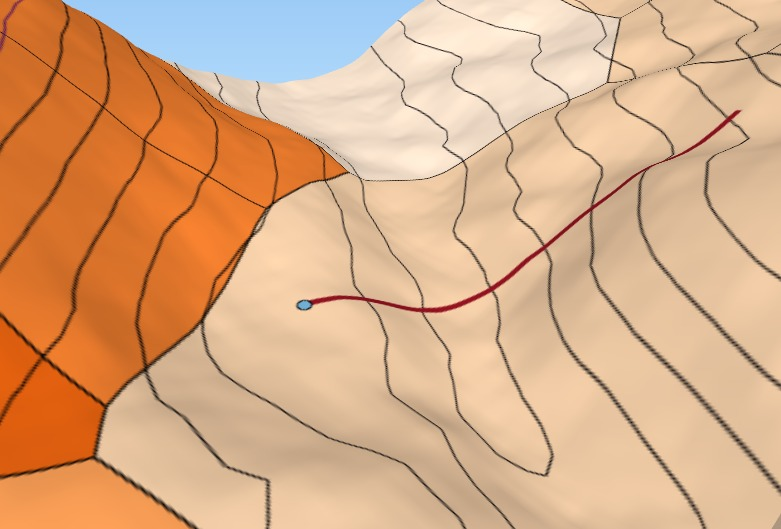
\includegraphics[width=0.4\linewidth]{img/Aversa}} \quad
\subfloat[]
{\label{fig:aversa-b}
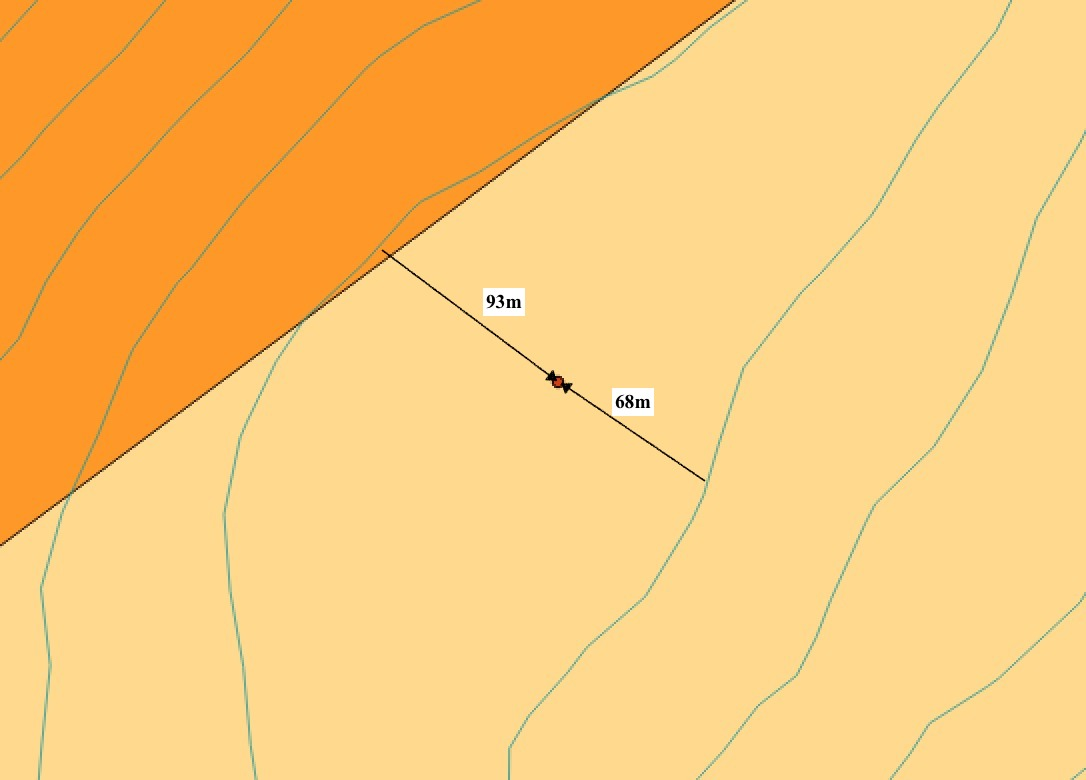
\includegraphics[width=0.38\linewidth]{img/Aversa2}} 
\caption[]{Stazione Ferroviaria di Aversa}\label{fig:aversa}
\end{figure}
\item \textbf{Vigliano d'Abruzzo}
\newline La stazione ferroviaria di Vigliano d'Abruzzo viene classificata dal nostro metodo in fascia \textit{Moderate} mentre \textit{ufficialmente} viene classificata in fascia \textit{High}. In figura \ref{fig:vigliano} è visibile come il  \textit{vettoreDirezionale} viene costruito considerando la curva di livello più vicina (a 38m) al punto che indica la stazione di Aversa mentre il pendio con una pendenza maggiore si riferisce alla curva di livello che dista 56m dal punto. Ragion per cui, il valore di \textit{exposure} ottenuto applicando il metodo proposto nella Sez. \ref{metodoNuovo} per questa stazione ferroviaria è tale da classificare erroneamente tale edificio in fascia \textit{Moderate}. 

\begin{figure}[bth]
\myfloatalign
\subfloat[]
{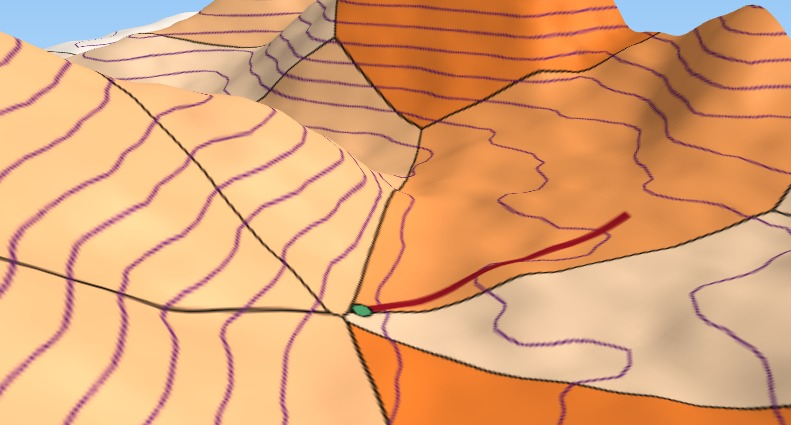
\includegraphics[width=0.45\linewidth]{img/Vigliano}} \quad
\subfloat[]
{\label{fig:aversa-b}
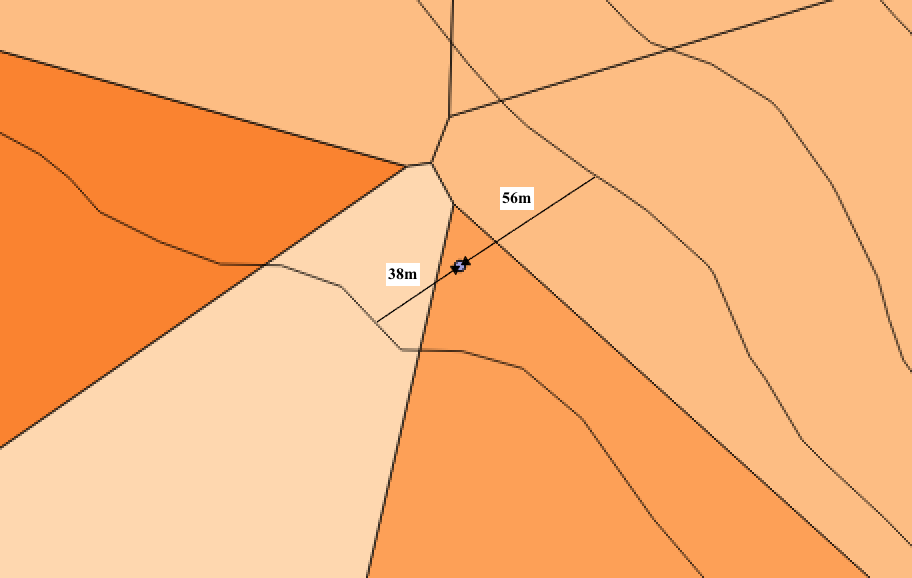
\includegraphics[width=0.38\linewidth]{img/Vigliano2}} 
\caption[]{Stazione Ferroviaria di Vigliano d'Abruzzo}\label{fig:vigliano}
\end{figure}
\end{itemize}

%----------------------------------
\section{Ranking e Valutazione delle linee ferroviarie}
\subsection{Discussione dei risultati ottenuti}
I risultati ottenuti applicando Il NMCE (vedi Sez.\ref{metodoLinee}) per la classificazione delle linee ferroviarie sono molto positivi, infatti si è osservato che la maggior parte dei segmenti che compongono le diverse linee ferroviarie hanno valori di \textit{exposure} corretti. Per la validazione di questi risultati è stato utilizzato il software QGIS e un suo plugin (vedi appendice \ref{qgis}) per la visualizzazione 3D di dati raster, in modo da poter verificare visivamente la correttezza dei valori di \textit{exposure} dei segmenti calcolati dal NMCE. \newline
 In alcuni casi il valore di \textit{exposure} dei segmenti in prossimità di una stazione sono in contrasto con la fascia assegnata a quest'ultima dal NMC. Questi casi corrispondono ai casi critici di cui abbiamo ampiamente parlato nelle sezioni \ref{analisicritica} e \ref{discussioneRisultati}.\\
Ad esempio la stazione di Aversa sappiamo essere stata classificata erronaemente nella fascia \textit{Moderate} dal NMC. Invece il NMCE classifica i segmenti in prossimità della stazione nella fascia \textit{High} (indicata con il colore rosso) come si evince dalla Fig.\ref{esempio1}. 
 
\begin{figure}[bth]
	\myfloatalign
	\subfloat[ Vista 2D della stazione di Aversa e della linea ferroviaria che l'attraversa]
	{\label{segmentiLinea}
		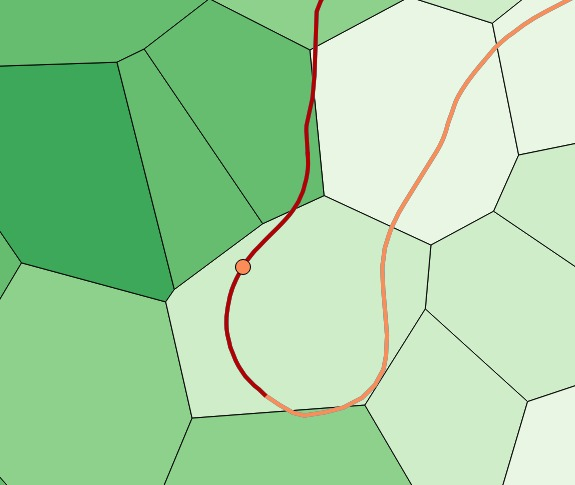
\includegraphics[width=.45\linewidth]{img/aversaLinea}} \quad
	\subfloat[Vista 3D della stazione di Aversa e della linea ferroviaria che l'attraversa ]
	{\label{mediaExposure}
		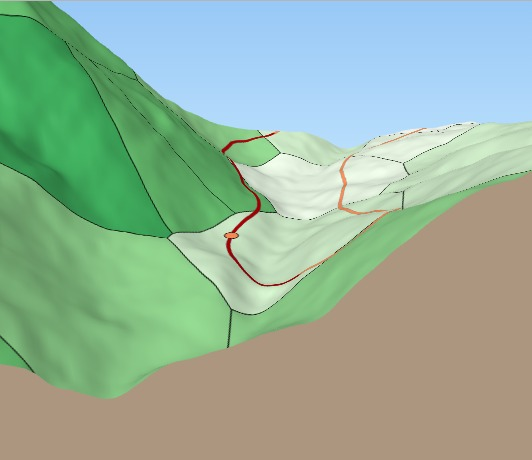
\includegraphics[width=.45\linewidth]{img/aversaLinea3}} 
	\caption[dove]{Vista 2D e 3D della stazione di Aversa e della linea ferroviaria che l'attraversa }
	\label{esempio1}
\end{figure}

Questo avviene perché l'\textit{exposure} del segmento viene determinato dalla media aritmetica dell'\textit{exposure} di tre punti ( vedi Sez.\ref{metodoLinee}), di conseguenza se ci fosse all'interno di un segmento un punto per il quale il calcolo dell'\textit{exposure} è stato compromesso, a causa delle limitazione del NMC  già discusse nella Sez.\ref{discussioneRisultati},  l'effetto di tale punto nel determinare il valore finale di \textit{exposure} del segmento verrebbe attenuato dagli altri punti all'interno di esso. \\
Il NMCE presenta una limitazione legata strettamente alle informazioni presenti nel \textit{dataset}, tale criticità corrisponde alla presenza di gallerie nelle linee ferroviarie. Il dataset utilizzato (vedi Sez.\ref{zone}) non possiede tali informazioni, dunque alcune tratte hanno segmenti che sono falsi positivi.\\
Ad esempio nella linea ferroviaria Pescara-Roma dal km 154 al km 157 la linea ferroviaria prosegue all'interno di una galleria. Tuttavia il NMCE non è a conoscenza di questa situazione e crede che la tratta continui arrampicandosi sul pendio, di conseguenza i segmenti che costituiscono la tratta hanno valori di \textit{exposure} altissimi. Di seguito in Fig.\ref{esempio2} si propongono le schermate 2D e 3D catturate mediante QGIS.
 
 \begin{figure}[bth]
 	\myfloatalign
 	\subfloat[ Vista 2D della tratta Pescara-Roma dal km 154 al 157]
 	{\label{2dPescaraRoma}
 		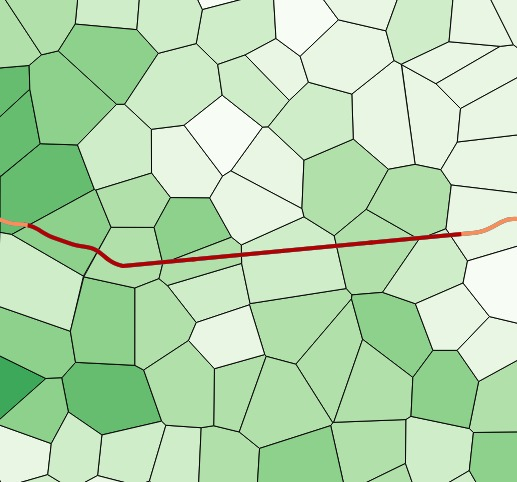
\includegraphics[width=.45\linewidth]{img/esempioGalleria2}} \quad
 	\subfloat[Vista 3D della tratta Pescara-Roma dal km 154 al 157 ]
 	{\label{3dPescaraRoma}
 		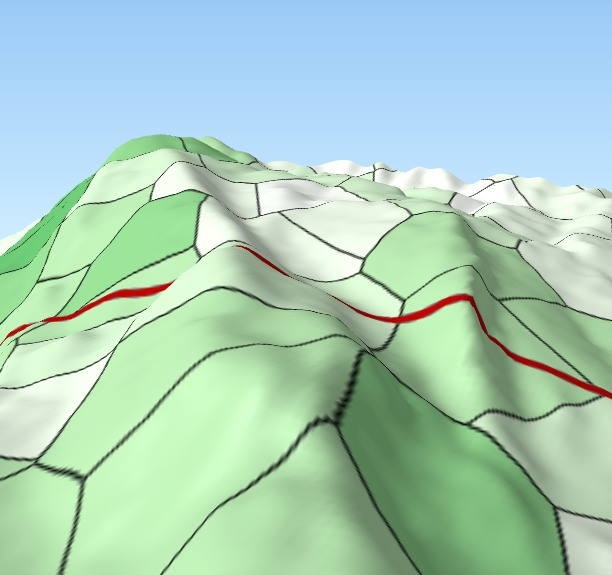
\includegraphics[width=.45\linewidth]{img/esempioGalleria3}} 
 	\caption[dove]{Vista 2D e 3D  della tratta Pescara-Roma dal km 154 al 157 }
 	\label{esempio2}
 \end{figure}
 